\documentclass[14pt,aspectratio=169]{beamer}

\usepackage{pgfpages}
\usepackage{fancyvrb}

\usepackage{tikz}
\usepackage{pgfplots}

\usepackage{minted}
\usemintedstyle{tango}

\usepackage{graphicx}

\usetheme{auriga}
\usecolortheme{auriga}

\setbeamercolor{background canvas}{bg=lightgray}

% define some colors for a consistent theme across slides
\definecolor{red}{RGB}{181, 23, 0}
\definecolor{blue}{RGB}{0, 118, 186}
\definecolor{gray}{RGB}{146, 146, 146}

\title{Web Development: \\ Using Color and Web Media}

\author{{\bf Gregory M. Kapfhammer}}

\institute[shortinst]{{\bf Department of Computer Science, Allegheny College}}

\begin{document}

{
  \setbeamercolor{page number in head/foot}{fg=background canvas.bg}
  \begin{frame}
    \titlepage
  \end{frame}
}

% Slide
%
\begin{frame}{Technical Question}
  %
  \hspace*{.25in}
  %
  \vspace*{.1in}
  %
  \begin{minipage}{4.5in}
    %
    \begin{center}
      %
      {\large How can I use HTML and CSS source code and media creation software to
      effectively add color and media such as images to a web site?}
      %
    \end{center}
    %
  \end{minipage}
  %
  \vspace{2ex}
  %
  \begin{center}
    %
    \small Let's learn how to combine CSS and HTML to create color and images!\\
    \small We will also explore the benefits of using external software to
    create media !\\
    \small Since web development in cumulative, please review all previous content!\\
    %
  \end{center}
  %
\end{frame}

% Slide
%
\begin{frame}{User Input with HTML5 Forms}
  %
  \begin{itemize}
    %
    \item Before HTML5, user input and form customization was limited; now
      multiple tags, CSS styling options, and services exist. Static sites
      present additional challenges!
      %
      \vspace*{-.15in}
      %
    \item Some examples of form components in HTML:
      %
      \begin{itemize}
        %
        \item Lists, radio buttons, and checkboxes
          %
        \item Form submission buttons and controls
          %
        \item Controls for input of text and file uploads
          %
      \end{itemize}
      %
      \vspace*{-.2in}
      %
    \item What type of content is best requested in a form?
      %
      \vspace*{-.2in}
      %
    \item What are not the most appropriate uses of a form?
      %
      \vspace*{-.2in}
      %
    \item What are the challenges associated with creating a form?
      %
  \end{itemize}
  %
\end{frame}

% Slide
%
\begin{frame}{The Lifecycle of Form Interaction}
  %
  \begin{itemize}
    %
    \item Does the web server provide a database for storage?
      %
      \vspace*{-.2in}
      %
    \item Does the web client support JavaScript or form validation?
      %
      \vspace*{-.2in}
      %
    \item The lifecycle of form creation and interaction:
      %
      \begin{itemize}
        %
        \item Developer creates a form and publishes to a web page
          %
        \item Developer connects the form to a data storage endpoint
          %
        \item Person views the form and submits the required content
          %
        \item The web client validates the form's current content
          %
        \item The web client transmits form content to the server
          %
      \end{itemize}
      %
      \vspace*{-.25in}
      %
    \item What are the challenges associated with creating a form?
      %
      \vspace*{-.25in}
      %
    \item What are the trade-offs associated with HTML forms?
      %
  \end{itemize}
  %
\end{frame}

% Slide
%
\begin{frame}{Using Formspree in Static Sites}
  %
  \begin{figure}
    \centering
    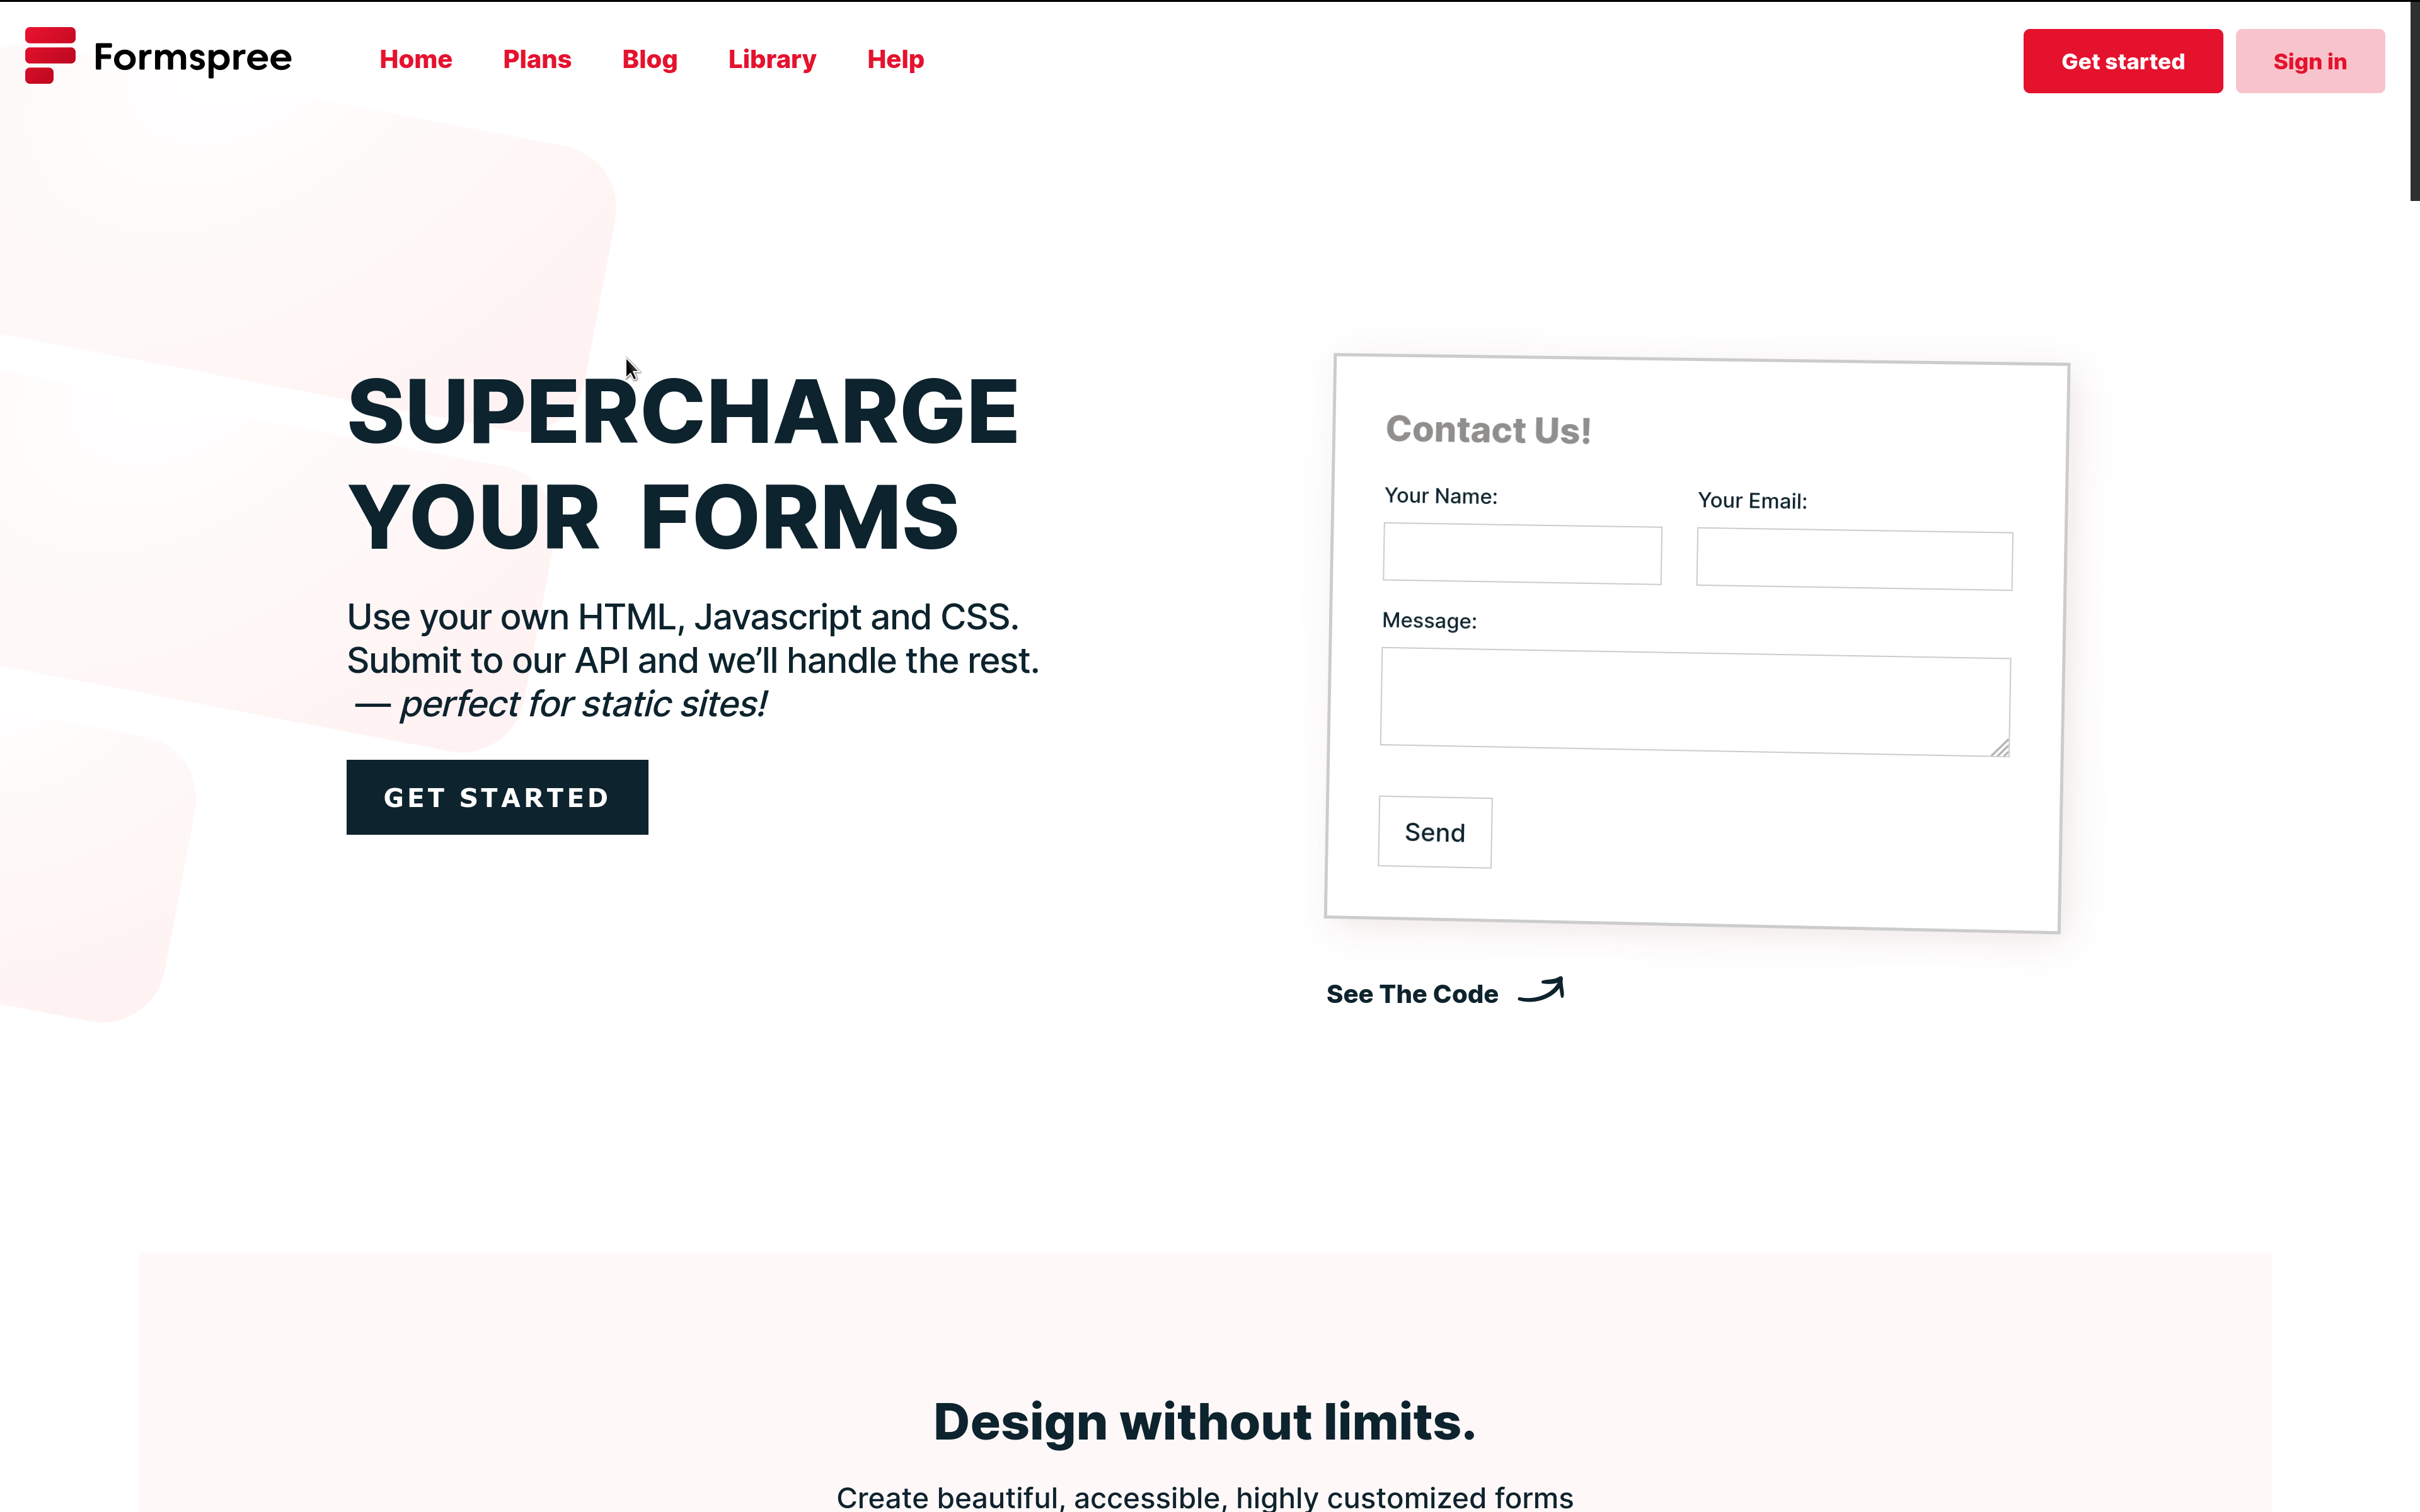
\includegraphics[scale=.08]{images/formspree.png}
    \caption{The figure's caption}
  \end{figure}
  %
\end{frame}

% Slide
%
\begin{frame}[fragile]
  \frametitle{Programming HTML Forms Using Formspree}
  \normalsize
  \begin{minipage}{6in}
    \vspace*{.1in}
    \begin{minted}[mathescape, numbersep=5pt, fontsize=\large]{html}
    <form
      action="https://formspree.io/
              gkapfham@
              allegheny.edu"
      method="POST">
      Share your Views!
      <input type="submit"
      value="Submit">
    </form>
    \end{minted}
  \end{minipage}
  %
\end{frame}

\end{document}
